
\documentclass{article}
\usepackage{graphicx}
\usepackage{booktabs}
\usepackage{geometry}
\geometry{a4paper, margin=1in}
\title{Rainfall Forecasting Report}
\author{Machine Learning Project}
\date{\today}

\begin{document}
\maketitle

\section{Introduction}
This report summarizes the results of rainfall forecasting in Selangor using machine learning techniques. 
The analysis includes model performance metrics and visualizations of the predictions.

\section{Model Comparison}
The following table shows the performance metrics for each model:

\begin{table}[h]
\centering
\caption{Model Performance Comparison}
\begin{tabular}{lccc}
\toprule
Model & RMSE & MAE & R\textsuperscript{2} \\
\midrule

\bottomrule
\end{tabular}
\end{table}

The best performing model is \textbf{dummy\_model}.

\section{Visualizations}
\subsection{Time Series of Rainfall}
\begin{figure}[h]
\centering
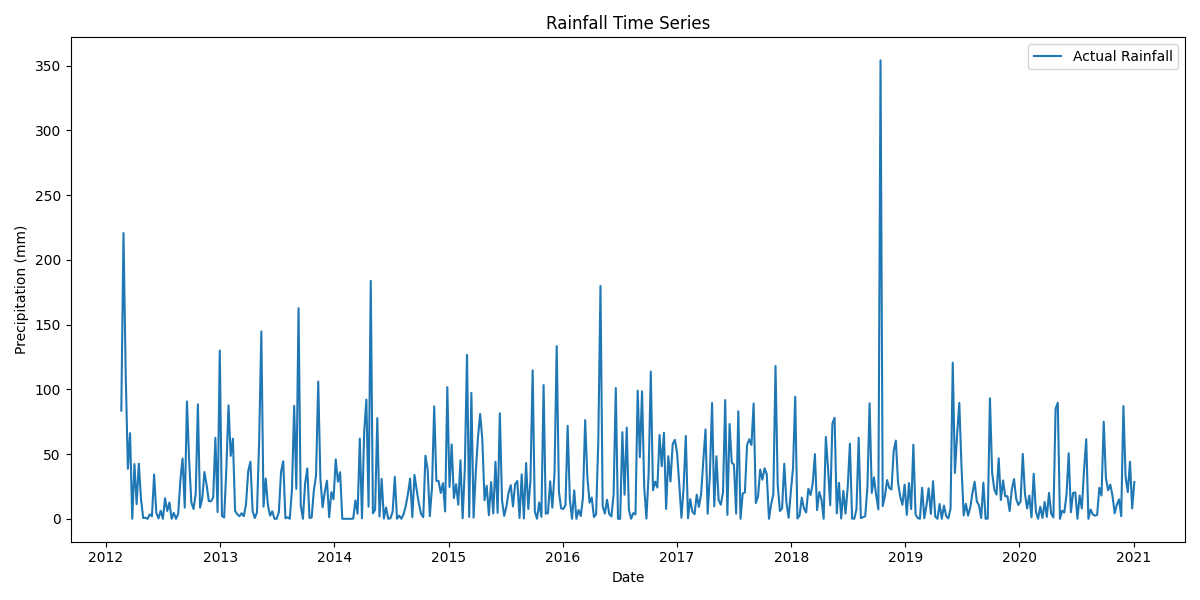
\includegraphics[width=0.8\textwidth]{figures/time_series.png}
\caption{Time Series of Actual Rainfall}
\end{figure}

\subsection{Prediction vs Actual}
\begin{figure}[h]
\centering
\includegraphics[width=0.8\textwidth]{figures/dummy_model_pred_vs_actual.png}
\caption{Predicted vs Actual Rainfall (dummy\_model)}
\end{figure}

\subsection{Model Comparison}
\begin{figure}[h]
\centering
\includegraphics[width=0.8\textwidth]{figures/model_comparison.png}
\caption{Model Performance Comparison}
\end{figure}

\end{document}
